\documentclass[border=10pt]{standalone}

\usepackage{tikz}
\usepackage{tikzsymbols}
\usetikzlibrary{calc,patterns,shapes.geometric}

\def\centerarc[#1](#2)(#3:#4:#5){\draw[#1] ($(#2)+({#5*cos(#3)},{#5*sin(#3)})$) arc (#3:#4:#5);}

\begin{document}
	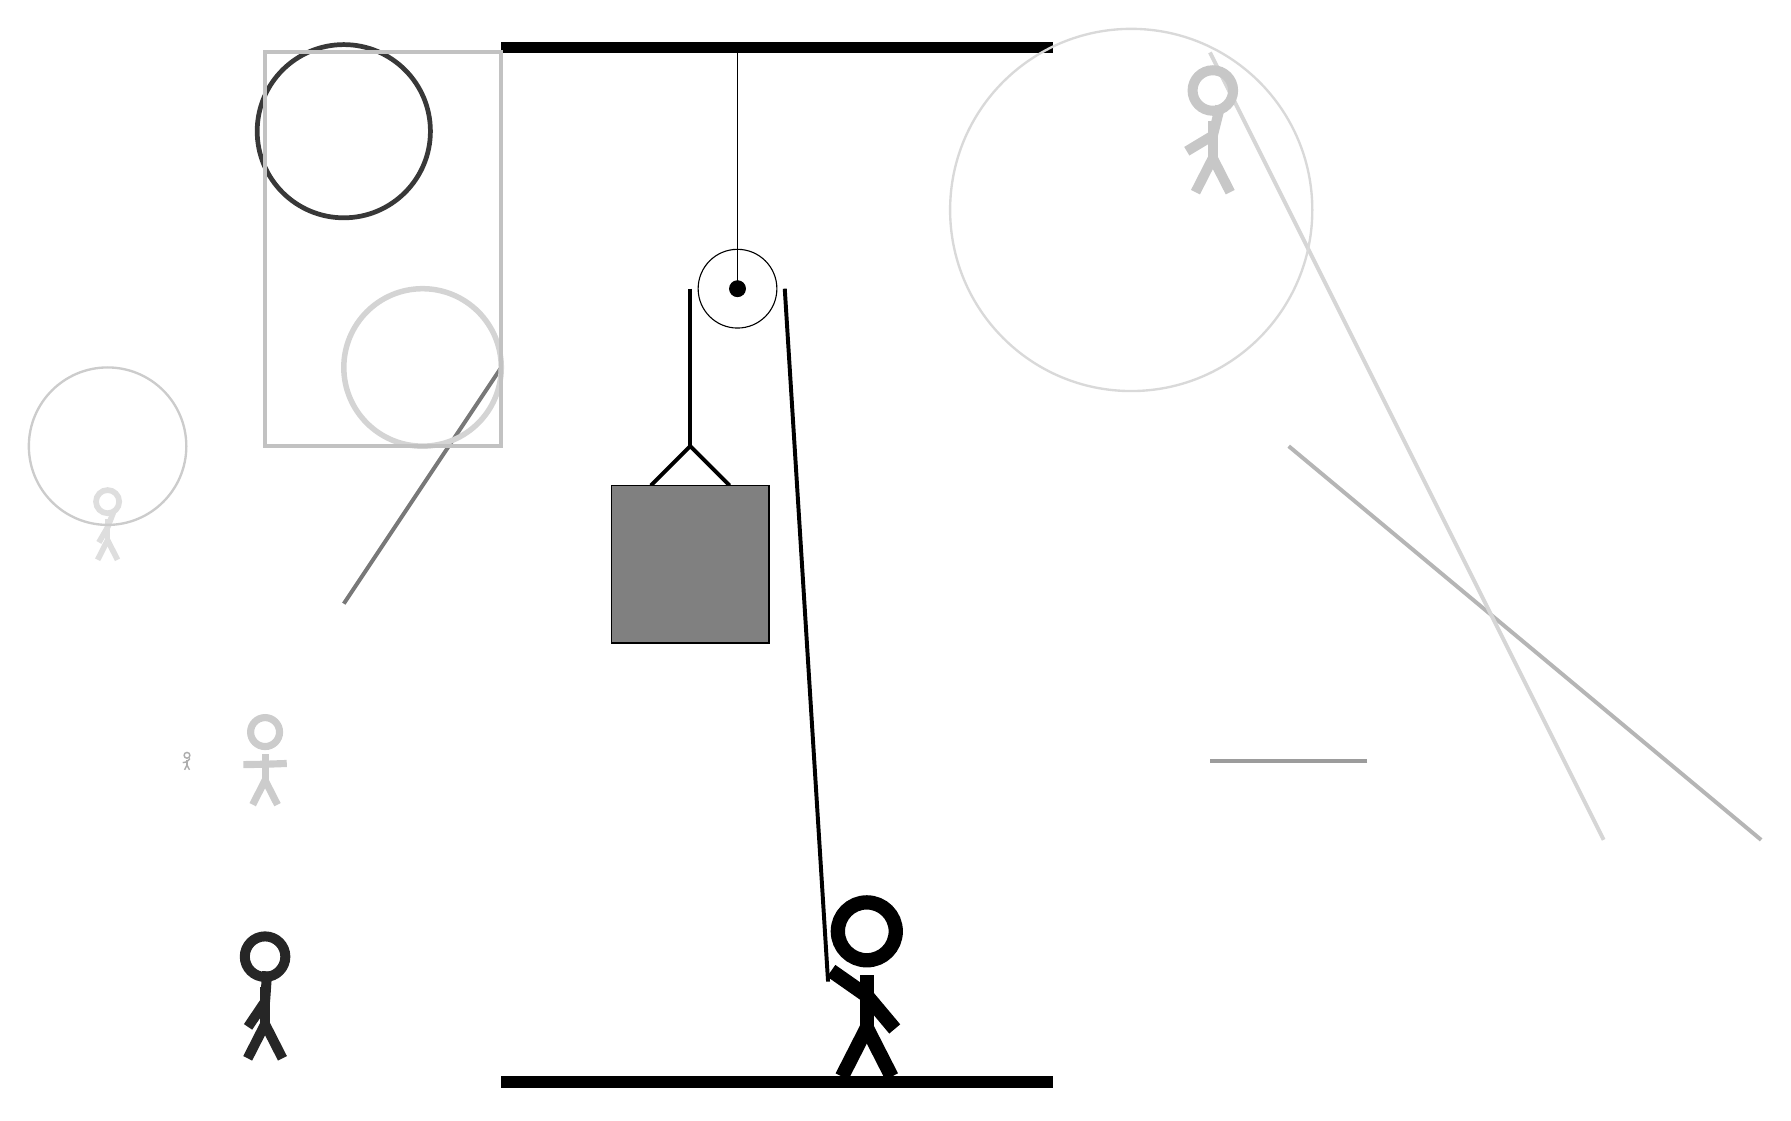
\begin{tikzpicture}
		%%%%% START %%%%%
		
		\draw[fill=black] (-2, 10) rectangle (5, 10.125);
		
		\draw (1, 7) circle (0.5);
		\draw[fill=black] (1, 7) circle (0.1);
		\draw (1, 10) -- (1, 7);
		
		\draw[line width=0.5mm] (-0.1, 4.5) -- (0.4, 5.0) -- (0.9, 4.5);
		\draw[fill=black!50] (-0.6, 4.5) rectangle (1.4, 2.5);
		
		\node[line width=0.6mm, color=black!13] at (-7, 4) {\Strichmaxerl[4][60][69]};
		
		\draw[line width=0.5mm, color=black!53](-4, 3) -- (-2, 6);
		\node[line width=0.4mm, color=black!20] at (-5, 1) {\Strichmaxerl[5][1][2]};
		\draw[line width=0.5mm, color=black!29](8, 5) -- (14, 0);
		\node[line width=0.6mm, color=black!85] at (-5, -2) {\Strichmaxerl[7][56][86]};
		\draw [line width=0.3mm, color=black!20](-7, 5) circle (1.0);
		\node[line width=0.7mm, color=black!32] at (-6, 1) {\Strichmaxerl[1][12][48]};
		\draw [line width=0.6mm, color=black!78](-4, 9) circle (1.1);
		\draw[line width=0.5mm, color=black!16](7, 10) -- (12, 0);
		\draw [line width=0.7mm, color=black!17](-3, 6) circle (1.0);
		
		\draw[line width=0.5mm, color=black!39](9, 1) -- (7, 1);
		\draw [line width=0.3mm, color=black!15](6, 8) circle (2.3);
		\draw[line width=0.5mm, color=black!24] (-2, 5) rectangle (-5, 10);
		\node[line width=0.3mm, color=black!22] at (7, 9) {\Strichmaxerl[7][31][76]};
		
		\draw[line width=0.5mm] (0.4, 7) -- (0.4, 5.0);
		\centerarc[line width=0.5mm](1, 7)(0:180:0.6);
		\draw[line width=0.5mm](1.6, 7) -- (2.15, -1.8);
		
		\node at (2.6, -1.9) {\Strichmaxerl[10][-35][-50]};
		
		\draw[fill=black] (-2, -3) rectangle (5, -3.15);
		
		%%%%% END %%%%%
	\end{tikzpicture}
\end{document}